\section{Description of solid breeder blankets}\label{sec:intro-blanket-description}

Before describing the solid breeder blanket and the design requirements, it is worth reviewing the major features of a fusion reaction and potential reactor. The current, worldwide choice for fusion reaction is deuterium-tritium (D-T). The choice is based on D-T having a high reaction probability at the lowest ion temperature, high energy yield, fuel availability, and reaction products (how harmless are the daughter products). The D-T cycle is

\begin{align}
	\mathrm{D} +~\mathrm{T}&\xrightarrow{}~^4\mathrm{He}+\mathrm{n}+17.58~\text{MeV} \label{eq:dt-reaction}
\end{align}

While Deuterium ($D$, or $^2$H), is a stable isotope and is naturally occuring in an average abundance of 0.015 mole percent in water on Earth. Tritium ($T$, or $^3$H), conversely, is radioactive with a half life of only about 12.32 years; naturally decaying as $\beta^-$ emitter (no $\gamma$ rays),

\begin{align}\label{eq:t-decay}
	\mathrm{T} \xrightarrow{}~^3\mathrm{He} + \beta^-
\end{align}
%~~~~~~~~~~~~~~~~~~~~~~~~~~~~~~~~~~~~~~~~~~~~~~~~



%~~~~~~~~~~~~~~~~~~~~~~~~~~~~~~~~~~~~~~~~~~~~~~~~
\subsection{Tritium breeding}

Owing to its short half life, any naturally occurring tritium would decay at such a rapid pace it can never accumulate. Because of this, it will need to be generated artificially (breeded) if it is to be used as a fuel in a fusion reactor. Fusion reactor designs receiving the most attention from the international community include a tritium breeding blanket as an integral component for maintaining self-sufficiency of the reaction. It is achieved with lithium. When natural lithium interacts with a neutron, its two most common isotopes have the following reaction

\begin{align}
	\mathrm{n}_\text{fast} + ~^7\mathrm{Li} &\xrightarrow ~\mathrm{n}+\alpha + \mathrm{T} -2.47~\text{MeV}\label{eq:Li7T}\\
	\mathrm{n}_\text{thermal} + ~^6\mathrm{Li} &\xrightarrow ~ \alpha + \mathrm{T} +4.78~\text{MeV} \label{eq:Li6T}
\end{align}

where we haved used the common short-hand of $\alpha$ in place of the helium nucleus. The cross-sections of the lithium reactions are given in Fig.~\ref{fig:li-xsects}

\begin{figure}
	\centering
	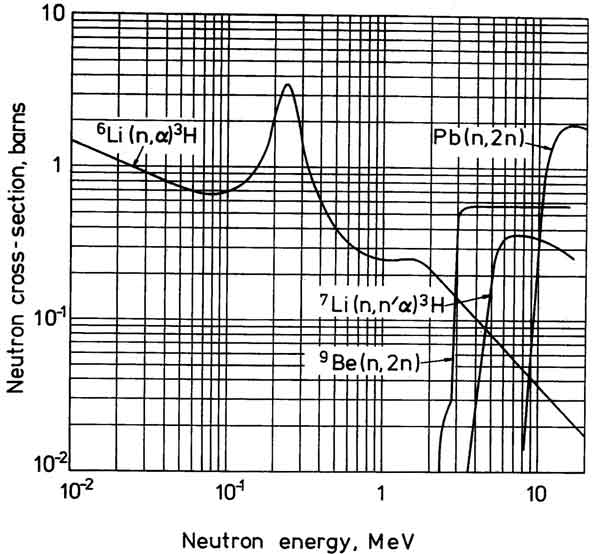
\includegraphics[width=0.8\textwidth]{chapters/figures/breeding_xsecs} 
	\caption{Cross-sections of various blanket materials. Note the threshold for the $^7$Li and neutron multiplying reactions.}
	\label{fig:li-xsects}
\end{figure}

Serendipitously, the D-T reaction itself produces a high energy neutron (see Eq.~\ref{eq:dt-reaction}). If we assume that $D$ is essentially limitless (on the scale of human consumption) and have access to abundant supplies of lithium, then if we complete the fuel cycle of neutron-lithium-tritium, we essentially have an inexhaustible energy source.

One classification of the efficacy of a breeding blanket is through the `tritium breeding ratio' of the fusion powerplant, defined as 

\begin{equation}
	\text{TBR} = \cfrac{\dot{N}^+}{\dot{N}^-}
\end{equation}

where $\dot{N}^+$ is the number of tritium atoms generated per unit time and $\dot{N}^-$ are the number of tritium atoms consumed per unit time.

For a DT cycle, $\dot{N}^- = $~number of fusion reactions in a plasma per unit time (each fusion reaction produces a single neutron). Therefore, for a DT cycle, we have a simplified definition that the tritium breeding ratio is the number of tritium atoms produced in the blanket per fusion neutron. In order to realize fusion as a commercial energy source, it is utterly crucial that the TBR of the plant design be greater than 1.

Clearly it is essential to engineer a device that surrounds the fusion reaction, captures the ejected neutron to breed tritium, and allows recovery of that tritium to attain self-sufficiency. Additionally, the blanket must also be capable of converting energy deposited from neutrons, $\gamma$s, and surface radiation from the plasma and then recovering the energy at high tempreatures for efficient power production in the fusion power plant.

Blanket designs have evolved significantly since their introducetion in the 1970s. Some features of current breeder designs will be discussed next.


% \chapter{Nuclear Design of the Blanket}
% \label{blanketDesign}
% The blanket contains:
% \begin{enumerate}
% \item Tritium breeding material (lithium in some form)
% \item Attenuating materials
% \item Neutron multipliers (in some designs)
% \item Coolant
% \item Structural material
% \item Reflector
% \item Insulators (in some designs)
% \end{enumerate}




%~~~~~~~~~~~~~~~~~~~~~~~~~~~~~~~~~~~~~~~~~~~~~~~~



%~~~~~~~~~~~~~~~~~~~~~~~~~~~~~~~~~~~~~~~~~~~~~~~~
\subsection{Solid breeder design}
Reference current styles of design. edge-on, etc.

% From TOFE-2014
The solid breeder in many current designs for ITER feature sub-module units of packed beds1. From the point of view of pebble bed thermomechanics, this has the advantage of producing units individually that can be tested and qualified to desired packing states (and therefore thermomechanics) during the design phase.

We aim to provide designers of packed beds with tools to understand how packing states may evolve from time-dependent phenomena (e.g. sintering, creep, pebble cracking, etc.). These phenomena may, for instance: decrease the effective thermal conductivity which will raise bed temperatures beyond initial predictions, produce isolated pebbles which will sinter and potentially decrease tritium release rates, or even the form gaps between pebble beds and containing structures leading to divergence from initial packing properties. 
%~~~~~~~~~~~~~~~~~~~~~~~~~~~~~~~~~~~~~~~~~~~~~~~~



%~~~~~~~~~~~~~~~~~~~~~~~~~~~~~~~~~~~~~~~~~~~~~~~~
\subsection{Material candidates and related phenomena}
Lithium can exist in the breeding blanket as either a liquid or a solid. We will limit the scope of our discussion entirely to the solid form. To date, most parties researching solid breeder devices are focusing on lithium orthosilicate (Li$_4$SiO$_4$) or lithium metatitanite (Li$_2$TiO$_3$) as candidate ceramics, though other candidate ceramics do still exist.

Solid breeders are always separately cooled by either water or helium flowing through coolant channels. 

Pure lithium is chemically active meaning safety is an issue. As an example, here are two reactions with oxygen along with their heats of formation
\begin{align*}
	2\mathrm{Li} + \frac{1}{2}\mathrm{O} &\rightarrow \mathrm{Li}_2\mathrm{O} - 142.75~\text{kCal/mol}\\
	2\mathrm{Li} + \mathrm{O} &\rightarrow \mathrm{Li}_2\mathrm{O}_2 - 151.9~\text{kCal/mol}
\end{align*}
note: a negative heat of formation means an exothermic reaction. Lithium will exothermically react with water (or air, concrete, or any moisture-containing materials) with high amounts of energy released. Of primary concern in lithium fires is the peak flame temperature. This will determine, to a large extent, whether many radioactive species become air-borne by vaporization. The flame temperature depends on many variables. Some investigations found it to be  about 2500 K which would cause some materials to melt but not vaporize.


% Neutron multipliers are needed to increase the breeding ratio, particularly in lithium compounds ({e.g.} Li$_4$SiO$_4$). Moreover they increase energy multiplication. Materials to act as neutron multipliers would be those that have large neutron multiplication cross sections (over large energy ranges). They react with (n,2n), (n,3n), or even (n, fission), however the fission reaction is obviously not desirable in a pure fusion reactor. Furthermore it is desirable that they have low neutron absorption and that they would have a favorable impact on energy multiplication. 

% The two most prominently analyzed neutron multipliers for a fusion reactor are beryllium and lead. Beryllium has a very high nuclide density while also being very light, with a high melting temperature, and high thermal conductivity. However it undergoes a 2-$\alpha$ reaction that causes trapped helium to swell the material. There is also a rarely occurring reaction with beryllium that generates tritium; it is frequent enough to cause a concern with contamination.
